% Chapter 3

\chapter{Morphology} % Main chapter title

\label{Chapter3} % For referencing the chapter elsewhere, use \ref{Chapter2} 


%----------------------------------------------------------------------------------------

\label{sec:Morphology}

Parvoviruses belong to the smallest of isometric viruses. A linear single-stranded DNA genome of about 5 kb is packaged into the virus capsid \cite{pmid4975639, pmid5264145, pmid5429749}. They are non-enveloped and their diameters range from 215 \r{A} (Penaeus stylirostris densovirus) to 255 \r{A} (CPV) \cite{pmid10497831, icvt}. 

The icosahedral nature of parvoviruses was shown unambiguously by a combination of electron microscopy (EM) and, latterly, X-ray crystallography \cite{pmid2006420}. Interpretation of the structural data gave rise to three distinct types of surface topology among parvoviruses (see Figure~\ref{Morphology}, p.~\pageref{Morphology}) \cite{pmid15795290}. The icosahedral twofold axes and the protrusions surrounding the icosahedral threefold axes display profound surface topology differences between each group. Types I and III comprise members of the \textit{Parvovirinae} subfamily described in Section~\ref{sec: The Parvovirinae subfamily}, see p.~\pageref{sec: The Parvovirinae subfamily}. They share in common the following surface features: a protrusion at the 3-fold axis, depressed regions between the 3-fold elevated regions at the 2-fold axis, and another depressed region encerceling the 5-fold axis. These two groups mainly differ in the shape of the 3-fold elevated region. 

Members of the genus \textit{Protoparvovirus}, as for example CPV, FPV, MVM, and PPV, represent the first topology group that is characterized by a single, relatively flat, pinwheel-shaped protrusion at the icosahedral threefold axes and a wider twofold dimple. The third topology group encompasses the AMDV, B19V, AAV2, AAV4, and AAV5 capsids, which show three distinct mounds at a distance of $\sim$20-26 \r{A} from the icosahedral threefold axes. In addition, the depression at the twofold axis appears to be slightly deeper, particularly for B19V \cite{pmid20375175, pmid12136130, tropism}. In contrast to the vertebrate parvoviruses, no large surface protrusions or depressions are present in \textit{Densovirus} capsids that appeared to be relatively spherical and featureless, adopting a second topology group \cite{pmid15769470, pmid9817847}.        


\begin{figure}[h] 
\centering
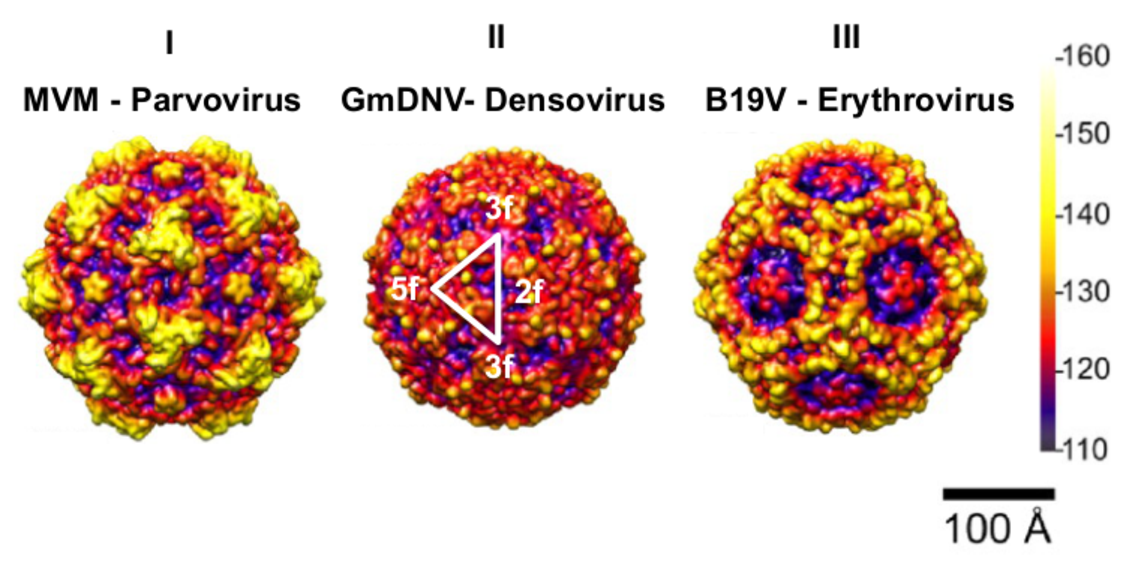
\includegraphics[width=0.9\textwidth]{Morphology}
\caption[Parvovirus surface topology groups]{Surface topology groups among members of the \textit{Parvoviridae} family. Stereo, depth cued (blue-red-yellow-white), and space-filling capsid surface illustration of representative members of the two subfamilies of the parvoviruses. Type viruses representing the three surface topology groups (I-III) and the genus to which they belong are indicated. A viral asymmetric unit bound (white triangle) is shown by a 2-fold (2f), two 3-folds (3f) and a 5-fold (5f) axis on the GmDNV image. A horizontal scale bar (100 \r{A}) for diameter measurement and a vertical color bar depicting color cueing as a function of particle radius in \r{A} are shown on the right hand side. These images were computed from atomic coordinates using the UCSF-Chimera program \cite{pmid15264254}, and all are rendered at the same resolution (7.9 \r{A}) and magnification. The figure was adapted from \cite{pmid20375175}.}
\label{Morphology}
\end{figure}

%The capsid surface of some, particularly invertebrate, parvoviruses appears to be smooth (Galleria mellonella densovirus, GmDNV) whereas others (Adeno-associated virus-2, AAV-2) are spiky at the 3- or 5-fold symmetry axes \cite{pmid10497831, icvt}.      


\nomenclature{GmDNV}{Galleria mellonella densovirus}
\nomenclature{DNA}{Deoxyribonucleic acid}
